\chapter{Espaces Métriques et Indexation par VP-Tree}
\label{chap:metriques_vptree}

\section{Espaces Métriques et Mesures de Dissimilarité}

\subsection{Définition Formelle d'un Espace Métrique}
Un espace métrique est un couple $(\mathcal{X}, d)$ où $\mathcal{X}$ est l'ensemble des descripteurs d'images et $d : \mathcal{X} \times \mathcal{X} \to \mathbb{R}^+$ satisfait aux quatre axiomes fondamentaux ($\forall \mathbf{x}, \mathbf{y}, \mathbf{z} \in \mathcal{X}$) :
\begin{enumerate}[nosep]
    \item \textbf{Non-négativité :} $d(\mathbf{x}, \mathbf{y}) \ge 0$.
    \item \textbf{Identité des indiscernables :} $d(\mathbf{x}, \mathbf{y}) = 0 \iff \mathbf{x} = \mathbf{y}$.
    \item \textbf{Symétrie :} $d(\mathbf{x}, \mathbf{y}) = d(\mathbf{y}, \mathbf{x})$.
    \item \textbf{Inégalité triangulaire :} $d(\mathbf{x}, \mathbf{z}) \le d(\mathbf{x}, \mathbf{y}) + d(\mathbf{y}, \mathbf{z})$.
\end{enumerate}
L'\textbf{inégalité triangulaire} est la condition sine qua non de l'élagage spatial métrique.

\subsection{Taxonomie des Métriques de Distance Implémentées}
Le module \texttt{cbir/distances/metrics.py} implémente six fonctions de distance :
\begin{itemize}[nosep]
    \item \textbf{Distance de Manhattan ($L_1$) :}
    \begin{equation}
        d_{L1}(\mathbf{x}, \mathbf{y}) = \sum_{i=1}^{d} |x_i - y_i|
    \end{equation}
    \item \textbf{Distance Euclidienne ($L_2$) :}
    \begin{equation}
        d_{L2}(\mathbf{x}, \mathbf{y}) = \sqrt{ \sum_{i=1}^{d} (x_i - y_i)^2 }
    \end{equation}
    \item \textbf{Distance du Chi-Deux ($\chi^2$) :}
    Idéale pour les histogrammes de fréquences, elle pondère les écarts par l'amplitude locale :
    \begin{equation}
        d_{\chi^2}(\mathbf{x}, \mathbf{y}) = \frac{1}{2} \sum_{i=1}^{d} \frac{(x_i - y_i)^2}{x_i + y_i + \epsilon} \quad (\epsilon = 10^{-10})
    \end{equation}
    \item \textbf{Intersection d'Histogrammes :} Mesure de recouvrement sur distributions normalisées :
    \begin{equation}
        d_{\cap}(\mathbf{x}, \mathbf{y}) = 1 - \sum_{i=1}^{d} \min(x_i, y_i) = \frac{1}{2} d_{L1}(\mathbf{x}, \mathbf{y})
    \end{equation}
    \item \textbf{Distance de Bhattacharyya :} Mesure de divergence multinomiale :
    \begin{equation}
        d_{\text{Bhatt}}(\mathbf{x}, \mathbf{y}) = -\ln\left( \sum_{i=1}^{d} \sqrt{x_i \cdot y_i} \right)
    \end{equation}
    \item \textbf{Distance Cosinus :} Mesure d'écart angulaire indépendante de la norme :
    \begin{equation}
        d_{\cos}(\mathbf{x}, \mathbf{y}) = 1 - \frac{\mathbf{x} \cdot \mathbf{y}}{\norm{\mathbf{x}}_2 \norm{\mathbf{y}}_2 + \epsilon}
    \end{equation}
\end{itemize}

\section{Le Fléau de la Dimensionnalité}

La recherche séquentielle naïve (\textit{brute-force}) calcule la distance entre la requête et les $n$ images de la collection : $T_{\text{exhaustif}} = \mathcal{O}(n \cdot d)$. Pour $n = 9~145$ et $d = 1~764$ (HOG), cela représente plus de $16$ millions d'opérations par requête, entraînant une latence supérieure à $4$ secondes.

Les structures classiques basées sur le découpage spatial cartésien (KD-Trees, R-Trees) échouent pour $d > 15$ en raison du \textbf{fléau de la dimensionnalité} \cite{bellman1957} :
\begin{enumerate}[nosep]
    \item Le volume d'une hypersphère inscrite de rayon $R$ rapporté à l'hypercube circonscrit tend vers zéro : $\lim_{d \to \infty} \frac{V_{\text{sphère}}(d, R)}{V_{\text{cube}}(d, 2R)} = 0$. La masse des données se concentre dans les coins.
    \item Phénomène de concentration des distances \cite{beyer1999} : $\lim_{d \to \infty} \frac{d_{\max} - d_{\min}}{d_{\min}} = 0$.
\end{enumerate}
Ces facteurs contraignent les KD-Trees à visiter toutes les feuilles de l'arbre, dégénérant en une recherche séquentielle avec une surcharge mémoire considérable.

\section{La Structure d'Indexation VP-Tree (\textit{Vantage-Point Tree})}

Le \textbf{VP-Tree} développé par Peter Yianilos \cite{yianilos1993} ne partitionne pas l'espace selon des axes cartésiens, mais exploite exclusivement les distances sphériques relatives à des points pivots nommés \textbf{points de vue} (\textit{Vantage Points}).

\begin{figure}[H]
    \centering
    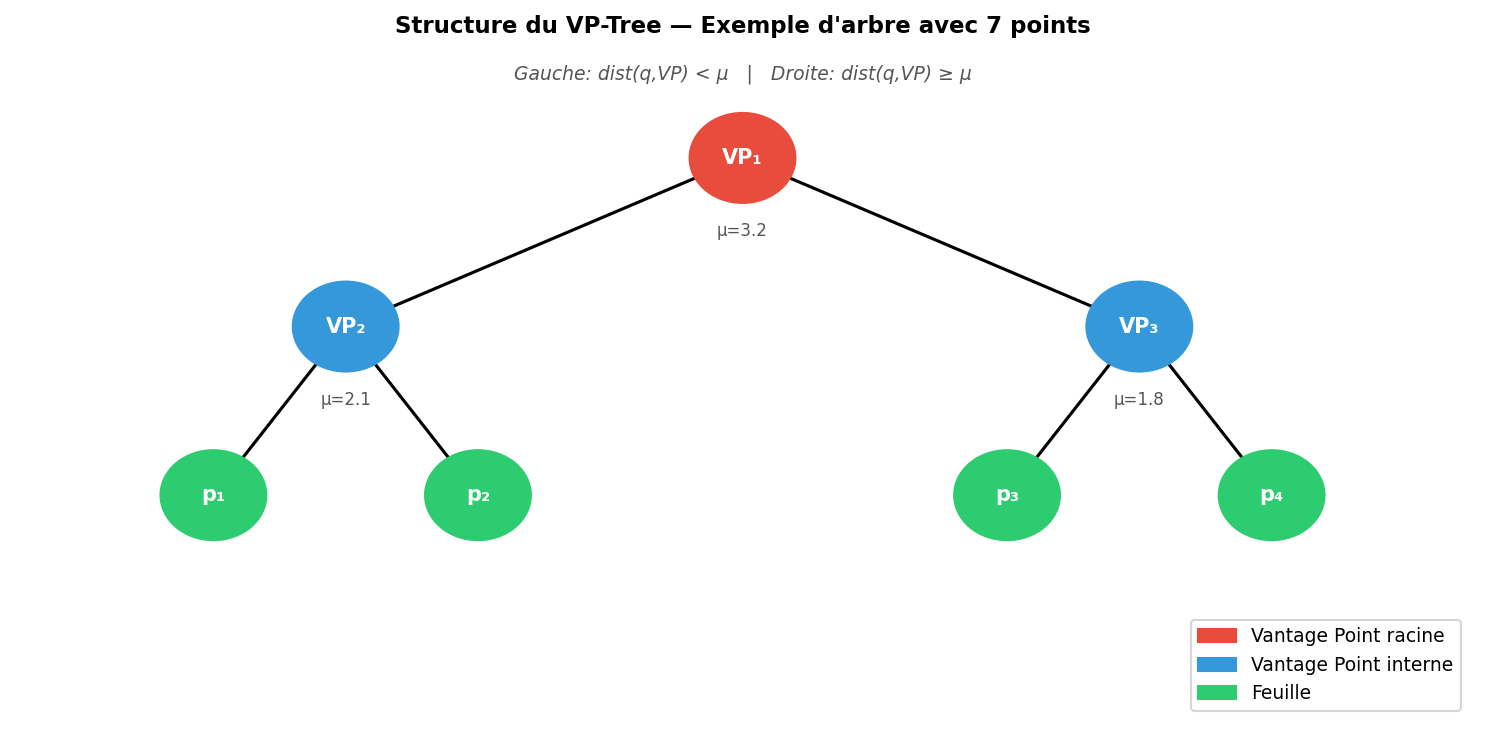
\includegraphics[width=0.82\textwidth]{figures/vptree_structure.png}
    \caption{Structure hiérarchique du VP-Tree : partitionnement sphérique équilibré autour du pivot via la distance médiane $\mu$.}
    \label{fig:vptree_principe}
\end{figure}

\subsection{Construction Récursive du VP-Tree}
Soit $\mathcal{S} = \{ (\text{id}_1, \mathbf{x}_1), \dots, (\text{id}_n, \mathbf{x}_n) \}$ un ensemble d'éléments. L'algorithme opère récursivement :
\begin{enumerate}[nosep]
    \item Choisir un point pivot $p_{\text{vp}} \in \mathcal{S}$ aléatoirement ou par maximisation de la variance des distances.
    \item Calculer l'ensemble des distances $D = \{ d(p_{\text{vp}}, x_i) \mid x_i \in \mathcal{S} \setminus \{p_{\text{vp}}\} \}$.
    \item Calculer la distance médiane $\mu = \text{médiane}(D)$.
    \item Scinder en deux sous-ensembles équilibrés : $\mathcal{S}_{\text{gauche}} = \{ x_i \mid d(p_{\text{vp}}, x_i) < \mu \}$ et $\mathcal{S}_{\text{droite}} = \{ x_i \mid d(p_{\text{vp}}, x_i) \ge \mu \}$.
    \item Récurser sur les deux sous-ensembles.
\end{enumerate}
L'arbre binaire produit possède une profondeur logarithmique $\lceil \log_2 n \rceil$ et une complexité de construction en $\mathcal{O}(n \log n)$.

\subsection{Théorèmes d'Élagage par l'Inégalité Triangulaire}
Soit une requête $q$, un rayon de recherche courant $\tau$ correspondant à la distance du $k$-ième plus proche candidat retenu dans le tas de priorité, et un nœud pivot $p_{\text{vp}}$ de médiane $\mu$.

\begin{theorem}[Élagage du Sous-arbre Gauche (Boule Interne)]
Tous les éléments $x$ du sous-arbre gauche vérifient $d(p_{\text{vp}}, x) < \mu$. Par l'inégalité triangulaire inversée :
\begin{equation}
    d(q, x) \ge d(q, p_{\text{vp}}) - d(p_{\text{vp}}, x) > d(q, p_{\text{vp}}) - \mu
\end{equation}
Si la condition suivante est satisfaite :
\begin{equation}
    d(q, p_{\text{vp}}) - \tau \ge \mu
\end{equation}
alors $\forall x \in \mathcal{S}_{\text{gauche}}, \; d(q, x) > \tau$. Le sous-arbre gauche tout entier est éliminé.
\end{theorem}

\begin{theorem}[Élagage du Sous-arbre Droit (Zone Externe)]
Tous les éléments $x$ du sous-arbre droit vérifient $d(p_{\text{vp}}, x) \ge \mu$. De même :
\begin{equation}
    d(q, x) \ge d(p_{\text{vp}}, x) - d(q, p_{\text{vp}}) \ge \mu - d(q, p_{\text{vp}})
\end{equation}
Si la condition suivante est satisfaite :
\begin{equation}
    \mu - d(q, p_{\text{vp}}) > \tau
\end{equation}
alors $\forall x \in \mathcal{S}_{\text{droite}}, \; d(q, x) > \tau$. Le sous-arbre droit est éliminé.
\end{theorem}

\subsection{Algorithme de Recherche $k$-NN}
La recherche maintient un tas-max (\textit{max-heap}) de capacité $k$. À chaque nœud visité, la distance $d(q, p_{\text{vp}})$ est calculée. Le sous-arbre le plus prometteur est exploré en premier (si $d(q, p_{\text{vp}}) < \mu$, la branche gauche est priorisée). Les bornes ci-dessus évitent l'exploration de la branche opposée dès lors qu'aucun point ne peut améliorer le rayon seuil $\tau$.

\subsection{Performances Empiriques : Accélération $\times 131$}
Sur le dataset Caltech-101 ($9~145$ images, descripteur \texttt{color\_rgb}, $d = 192$, $k = 20$), le VP-Tree apporte un gain spectaculaire :

\begin{table}[H]
    \centering
    \caption{Comparatif de performance : Recherche Exhaustive versus VP-Tree}
    \label{tab:vptree_gain}
    \begin{tabular}{lccc}
        \toprule
        \textbf{Indicateur} & \textbf{Recherche Exhaustive} & \textbf{Index VP-Tree} & \textbf{Facteur de Gain} \\
        \midrule
        Temps de recherche moyen & $4~198$ ms & \textbf{32 ms} & \textbf{$\times 131$ plus rapide} \\
        Comparaisons de vecteurs & $9~145$    & \textbf{21}    & \textbf{99,77\% d'élagage} \\
        Exactitude du rappel     & 100\%      & 100\%          & Préservation parfaite \\
        Taille sur disque        & —          & 7,7 Mo         & Négligeable \\
        \bottomrule
    \end{tabular}
\end{table}

\begin{figure}[H]
    \centering
    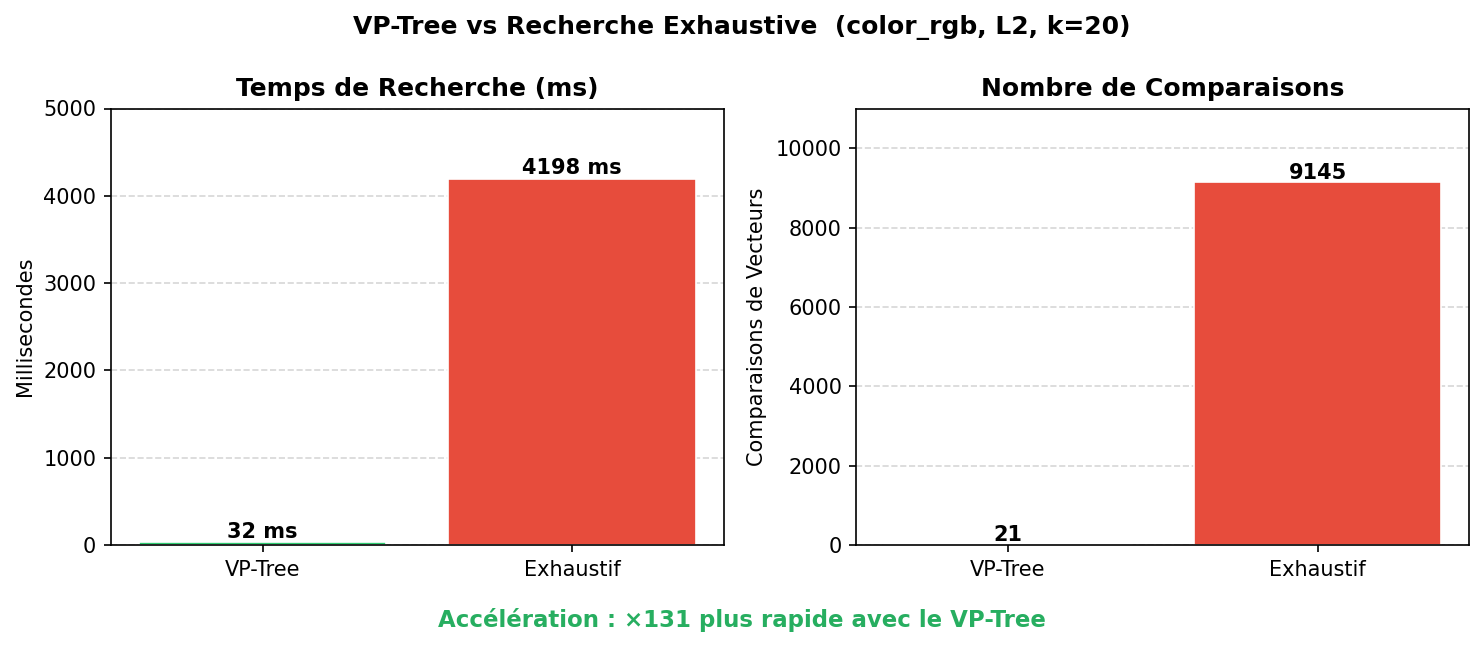
\includegraphics[width=0.82\textwidth]{figures/vptree_comparison.png}
    \caption{Comparatif direct VP-Tree vs Recherche Exhaustive : temps de latence et volume de comparaisons.}
    \label{fig:vptree_chart_compact}
\end{figure}
